\begin{frame}[c]{Datentransfer}
	\usetikzlibrary{shapes.geometric, arrows}
	\tikzstyle{normalArrow} = [thick,->,>=stealth, shorten <= 1.0cm, shorten >= 1.0cm]
	\begin{tikzpicture}[scale=0.7, transform shape]%
		\onslide<1->{
		\draw (0,0) circle (1.4) [path picture={ 
				\node at (path picture bounding box.center){
					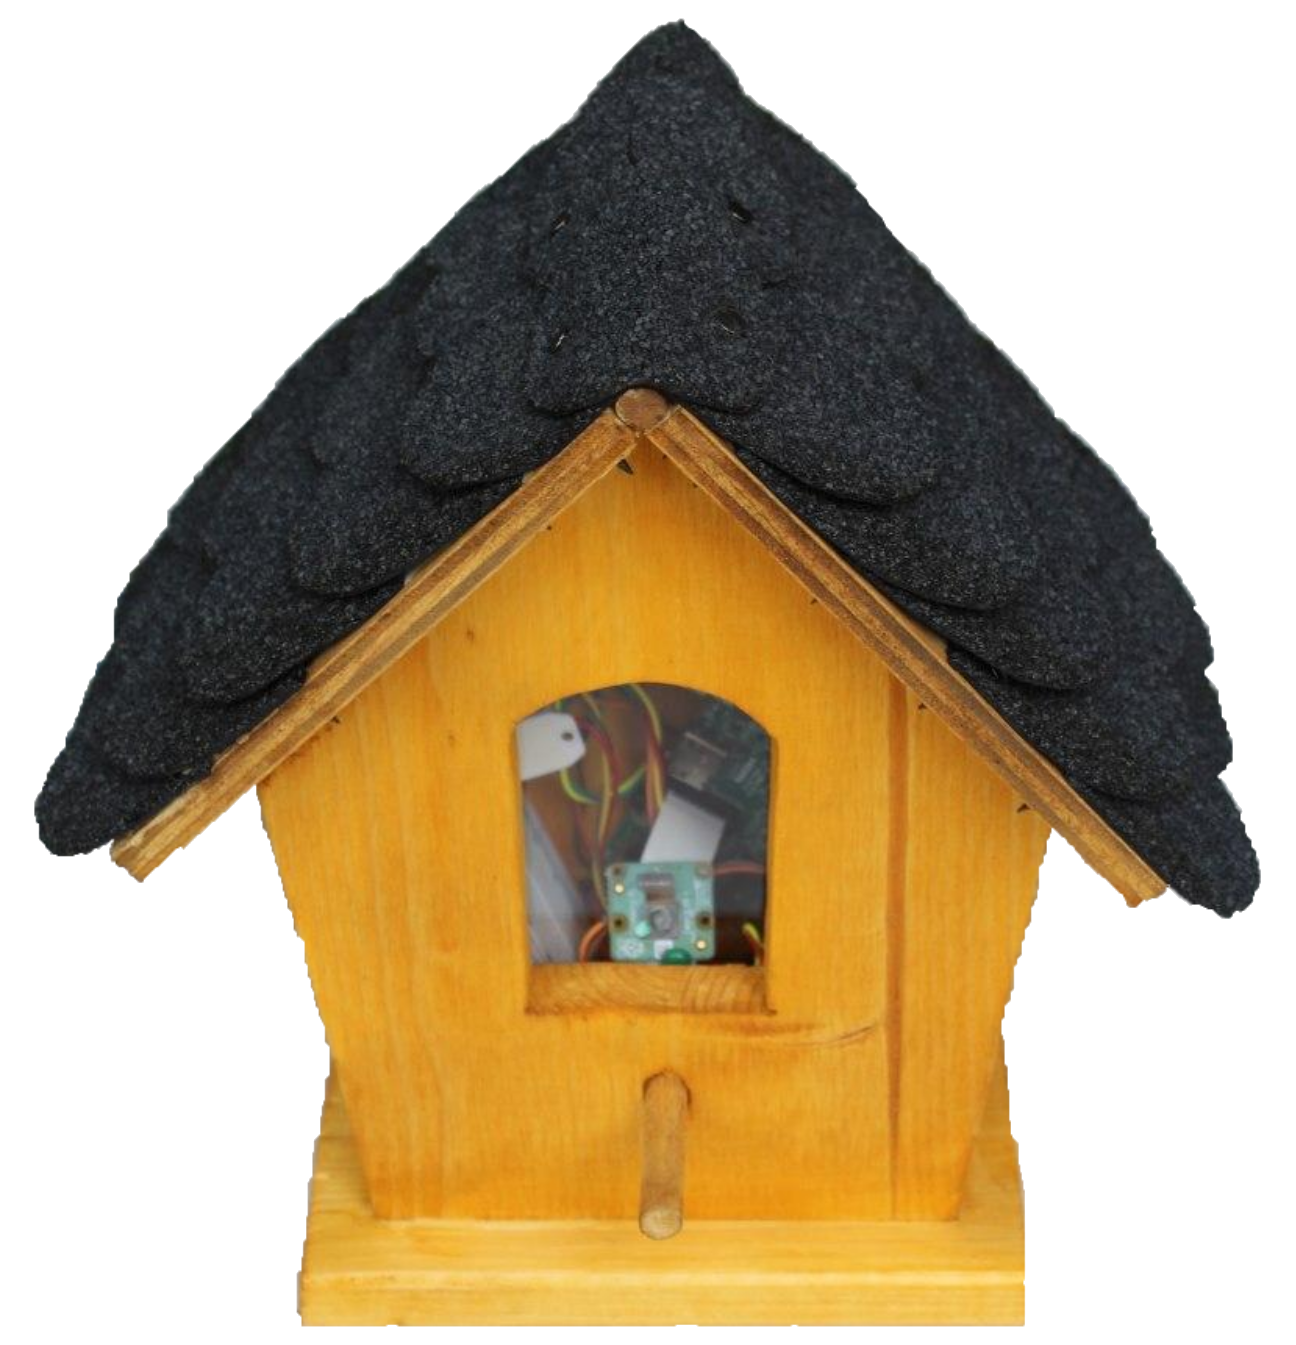
\includegraphics[height=2.8cm]{picture/wetterstation.png}};
			}, line width=1] node (A) {};
		\node (a) at (0, -2) {Mikroprozessor};
		}
		\onslide<2->{
		\draw (A)++(2.25,-4) [fill=black!10] rectangle ++(3.5,8.5);
		\node (b) at (4, 4) {Datentransfer};
		\draw (A)++(4,2) circle (1.4) [path picture={ 
				\node at (path picture bounding box.center){
					
\includegraphics[width=2.8cm]{picture/mariadb.png}};
			}, line width=1] node (C) {};
		\draw (A)++(4,-2) circle (1.4) [path picture={ 
				\node at (path picture bounding box.center){
					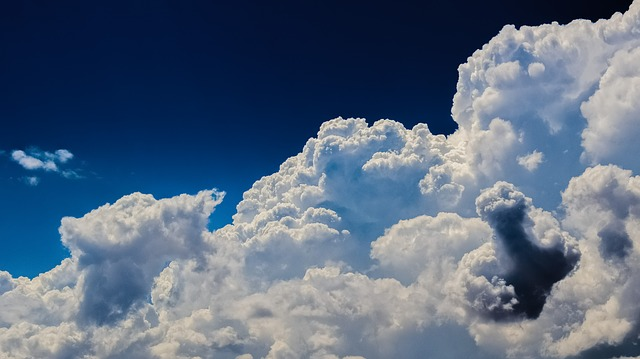
\includegraphics[height=2.8cm]{picture/clouds.jpg}};
			}, line width=1] node (D) {};
		\draw [normalArrow] (A) -- (C);
		\draw [normalArrow] (A) -- (D);
	}
		\onslide<3->{
		\draw (A)++(8,0) circle (1.4) [path picture={ 
				\node at (path picture bounding box.center){
					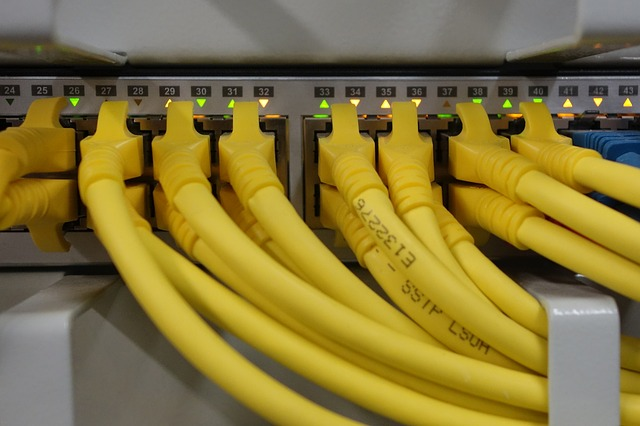
\includegraphics[height=2.8cm]{picture/network.jpg}};
			}, line width=1] node (E) {};
		\node (e) at (8,-2) {Server};
		\draw [normalArrow] (C) -- (E);
		\draw [normalArrow] (D) -- (E);
	}
		\onslide<4>{
		\draw (A)++(10.50,-4) [fill=black!10] rectangle ++(3.5,8.5);
		\node (D) at (12.25, 4) {Auswertung};
		\draw (A)++(11,0.75) rectangle ++(2.5,2.5) [path picture={ 
				\node at (path picture bounding box.center){
					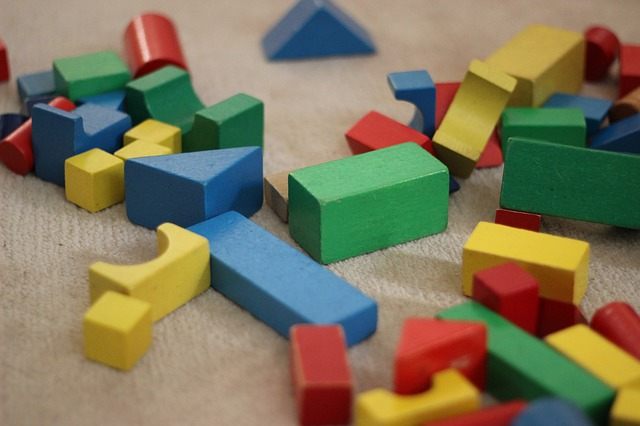
\includegraphics[height=2.5cm]{picture/building_blocks.jpg}};
			}, line width=1] node (F) {};
		\draw (A)++(11,-3.25) rectangle ++(2.5,2.5) [path picture={ 
				\node at (path picture bounding box.center){
					
\includegraphics[height=2.0cm]{picture/telegram.png}};
			}, line width=1] node (G) {};
		\draw [normalArrow] (E) -- (12,2);
		\draw [normalArrow] (E) -- (12,-2);
	}
	\end{tikzpicture}
\end{frame}
